\documentclass[12pt,aspectratio=169]{beamer}
\usetheme{Rochester}
\setbeamertemplate{navigation symbols}{}
\usecolortheme{default}
\usefonttheme{professionalfonts}

\usepackage[utf8]{inputenc}
\usepackage{xcolor}
\usepackage{fancyvrb}

\title{LTLSpec}
\subtitle{An extensible LTL verifier for distributed systems}
\author{Eric Conlon, Yanze Li, Tarcisio Teixeira}
\date{2021-12-07}

\begin{document}

\frame{\titlepage}

\begin{frame}
\frametitle{What is Runtime Verification?}
\begin{itemize}
  \item Want to know that a distributed system adheres to some spec
  \item Check spec against execution traces
  \newline (local/global, online/offline, incremental/batch)
  \item Best you can say: hasn't gone wrong yet
  \item But that's still pretty useful!
\end{itemize}
\end{frame}

\begin{frame}
\frametitle{Our project}
\begin{itemize}
  \item Implemented a runtime verifier for Linear Temporal Logic (LTL)
  \item Implemented several actor (message-passing) systems
  \item Defined an LTL theory for each system
  \item Verified execution traces of those systems
\end{itemize}
\end{frame}

\begin{frame}
\frametitle{Our assumptions}
\begin{itemize}
  \item Possible to gather local or global traces of actions/messages in a distributed system
  \item Traces don't violate causality
  \item Traces start at the beginning of execution
  \item Domains of quantification are finite (per-world)
\end{itemize}
\end{frame}

\begin{frame}
\frametitle{Example system: Ping}
\begin{itemize}
  \item Group of actors send \texttt{Ping} messages and respond with \texttt{Pong} messages
  \item We want this responsiveness property to hold:
  \begin{itemize}
    \item "Whenever I send a \texttt{Ping}, I eventually receive a \texttt{Pong}"
    \item Not enough that a \texttt{Pong} was sent to me, I need to receive it!
    \newline (Can define program correctness in presence of faulty environment)
    \item Need to formally specify this property to check it...
  \end{itemize}
\end{itemize}
\end{frame}

\begin{frame}
\frametitle{Example traces: Ping}
\begin{itemize}
  \item Observing global events as \texttt{(viewpoint, action)}
  \item Good trace (demonstrates responsiveness)
  \begin{itemize}
    \item \texttt{(Alice, Send Ping to Bob)}
    \item \texttt{(Bob, Recv Ping from Alice)}
    \item \texttt{(Bob, Send Pong to Alice)}
    \item \texttt{(Alice, Recv Pong from Bob)}
  \end{itemize}
  \item Bad trace (violates responsiveness): drop the \texttt{Recv Pong from Bob}
\end{itemize}
\end{frame}

\begin{frame}
\frametitle{What is Linear Temporal Logic (LTL)?}
\begin{itemize}
  \item World-relevant propositional logic
  \item Atomic propositions: \texttt{P}, \texttt{Q}
  \item Standard connectives: $\land$, $\lor$, $\neg$, $\implies$
  \item Modal connectives:
  \begin{itemize}
    \item $\Box$ \texttt{P} means \texttt{P} holds in \textit{all} accessible worlds
    \newline (\texttt{P} will \texttt{Always} be true, including now)
    \item $\Diamond$ \texttt{P} means \texttt{P} holds in \textit{some} accessible world
    \newline (\texttt{P} will \texttt{Eventually} be true, possibly now)
  \end{itemize}
  \item Expressive enough to capture our Ping-Pong property!
  \newline (...\texttt{Eventually} receive a \texttt{Pong}...)
\end{itemize}
\end{frame}

\begin{frame}
\frametitle{Making LTL useful}
\begin{itemize}
  \item Add data variable quantification (\texttt{LTL-FO+})
  \begin{itemize}
    \item Can write propositions about all values of some type
    \begin{itemize}
      \item $\forall$ \texttt{(x:T), P(x)}
      \item $\exists$ \texttt{(x:T), P(x)}
    \end{itemize}
    \item First order - no quantifying over propositions/types, just values
    \item Ping example: property can quantify over all \texttt{Ping} messages
  \end{itemize}
  \item Add user-defined atomic props and quantification
  \item Declare types, atomic props, and axioms in a user-defined "theory"
\end{itemize}
\end{frame}

\begin{frame}
\frametitle{Example theory: Ping}
  {\fontsize{10}{12}\selectfont
    \begin{Verbatim}[commandchars=\\\{\},codes={\catcode`$=3}]
\textcolor{black}{(*} \textcolor{black}{A ping request sent by an actor} \textcolor{black}{*)}
\textcolor{blue}{SentPing} \textcolor{darkgray}{:} \textcolor{cyan}{Set}
\textcolor{black}{(*} \textcolor{black}{A pong response received by an actor} \textcolor{black}{*)}
\textcolor{blue}{RecvPong} \textcolor{darkgray}{:} \textcolor{cyan}{Set}

\textcolor{black}{(*} \textcolor{black}{Characterizes a request-response pair} \textcolor{black}{*)}
\textcolor{teal}{IsPingPong} \textcolor{darkgray}{:} \textcolor{blue}{SentPing} \textcolor{darkgray}{$\rightarrow$} \textcolor{blue}{RecvPong} \textcolor{darkgray}{$\rightarrow$} \textcolor{cyan}{Prop}

\textcolor{black}{(*} \textcolor{black}{Every ping request eventually gets a pong response} \textcolor{black}{*)}
\textcolor{purple}{isResponsive} \textcolor{darkgray}{:} 
  \textcolor{teal}{$\Box$} \textcolor{darkgray}{(}\textcolor{teal}{$\forall$} \textcolor{darkgray}{(}\textcolor{red}{m1} \textcolor{darkgray}{:} \textcolor{blue}{SentPing}\textcolor{darkgray}{)}\textcolor{darkgray}{,} 
    \textcolor{teal}{$\Diamond$} \textcolor{darkgray}{(}\textcolor{teal}{$\exists$} \textcolor{darkgray}{(}\textcolor{red}{m2} \textcolor{darkgray}{:} \textcolor{blue}{RecvPong}\textcolor{darkgray}{)}\textcolor{darkgray}{,} 
      \textcolor{teal}{IsPingPong} \textcolor{purple}{m1} \textcolor{purple}{m2}\textcolor{darkgray}{)}\textcolor{darkgray}{)}
\end{Verbatim}

  }
\end{frame}

\begin{frame}
\frametitle{Verification is a conversation (1/2)}
\begin{itemize}
  \item Verifier only understands LTL connectives
  \begin{itemize}
    \item Doesn't understand user-defined types and props
    \item Doesn't understand worlds (trace elements) or values
  \end{itemize}
  \item For each domain require user-defined "bridge"
  \item Bridge for Ping system knows these parts
  \begin{itemize}
    \item Can enumerate all \texttt{SentPing} values in a world
    \item Can determine if two values satisfy \texttt{IsPingPong}
  \end{itemize}
  \item Driver feeds worlds to verifier, verifier works with the bridge to interpret propositions
\end{itemize}
\end{frame}

\begin{frame}
\frametitle{Verification is a conversation (2/2)}
  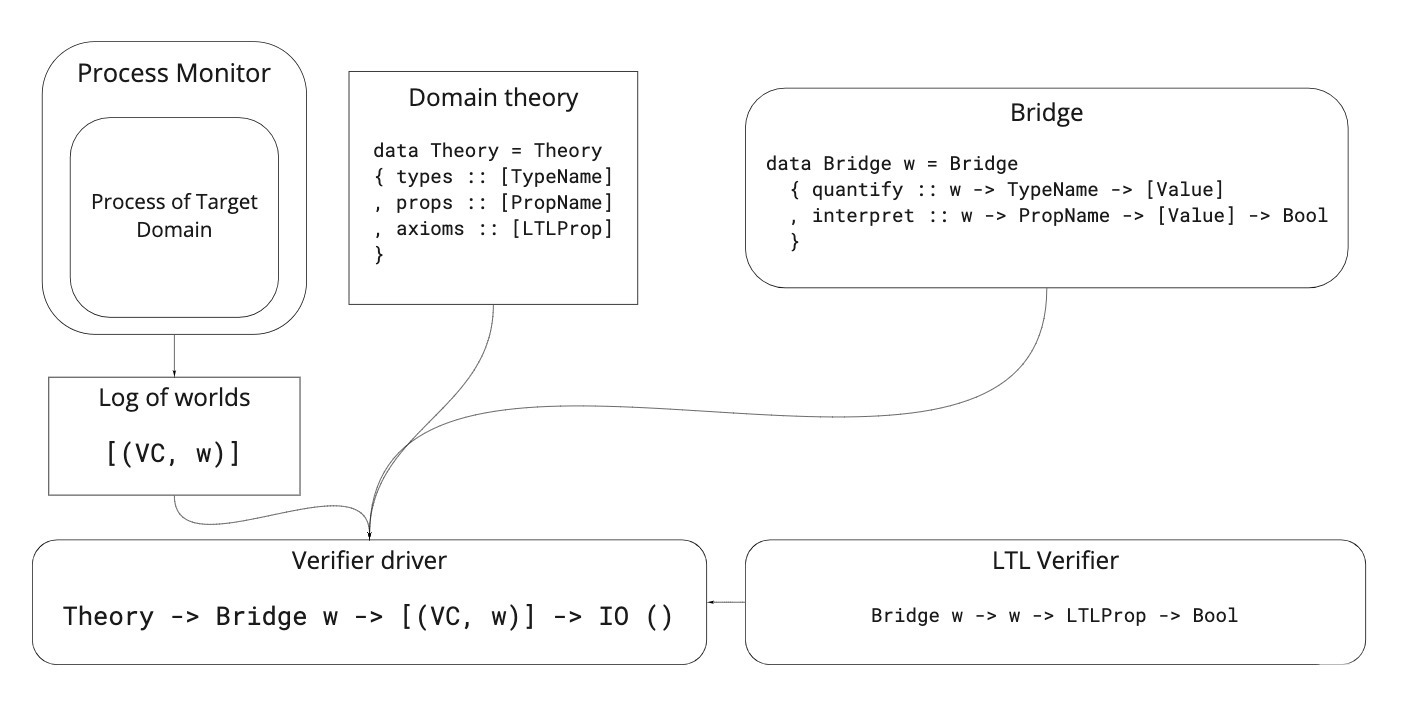
\includegraphics[scale=0.27]{diagram.jpg}
  \centering
\end{frame}

\begin{frame}
\frametitle{Encountering the infinite problem}
\begin{itemize}
  \item When testing, you only have \textit{finite} traces
  \item Modal connectives only have meaning on \textit{infinite} traces
  \item Can you say something \texttt{Always} happens?
  \item Can't verify a liveness property with a finite trace... Or can you?
  \item Trick: allow users to reason outside the logic about ALL future worlds
\end{itemize}
\end{frame}

\begin{frame}
\frametitle{Solving the infinite problem with truncation}
\begin{itemize}
  \item User bridge can tell the verifier that after this world
  \begin{itemize}
    \item Some set of types will have empty quantification
    \item Some set of atomic props will have constant values
  \end{itemize}
  \item This lets you prove responsiveness for quiescent systems
  \item For some props the best you can say is you can't prove or disprove them
  \item Not arbitrary: these criteria ensure no additional reduction is necessary
  \item (Some fragment of a higher-order 3-valued logic...)
\end{itemize}
\end{frame}

\begin{frame}
\frametitle{Example truncation: Ping}
\begin{itemize}
  \item \texttt{isResponsive :}
  \newline $\Box$ \texttt{(}$\forall$ \texttt{m1:SentPing,} $\Diamond$ \texttt{(}$\exists$ \texttt{m2:RecvPong, IsPingPong m1 m2))}
  \item No messages in flight or in mailbox $\rightarrow$ no more actions
  \item No more actions $\rightarrow$ \texttt{SentPing} and \texttt{RecvPong} types have empty quantification
  \item \texttt{IsPingPong} atomic prop is always a pure function of its arguments (regardless of world)
  \item Result: can evaluate responsiveness on any trace
\end{itemize}
\end{frame}

\begin{frame}
\frametitle{Evaluation (1/2)}
\begin{itemize}
  \item Implemented verifier, domains, and actor systems in Haskell
  \item Defined messages, roles, and actors for three domains:
  \begin{itemize}
    \item Ping, Chat System, and Dining Philosophers
  \end{itemize}
  \item Ran these in our actor framework with multi-threading and STM
  \begin{itemize}
    \item Implementation and STM semantics ensure trace order does not violate causality
    \item Wait for quiescence to ensure total trace collection
    \item Future work: introduce network faults (abstracted but not implemented)
  \end{itemize}
\end{itemize}
\end{frame}

\begin{frame}
\frametitle{Evaluation (2/2)}
\begin{itemize}
  \item Primary concerns: Syntax, Semantics, and Correctness
    \begin{itemize}
      \item Defined interfaces that generalize well
      \item Collected traces and verified axioms of each theory
      \item The tests pass... And we never write bugs!
    \end{itemize}
  \item Secondary concern: Performance
    \begin{itemize}
      \item Passable with naive interpreter - not stress-tested
      \item Want safe-for-space machine, term graph deduplication, predicate pushdown...
    \end{itemize}
\end{itemize}
\end{frame}

\begin{frame}
\frametitle{Thanks!}
\begin{itemize}
  \item See the repo: \url{https://github.com/ejconlon/ltlspec}
\end{itemize}
\end{frame}

\end{document}
